

{\subsection{What is \LaTeX?}
LaTeX (pronounced \enquote{Lay-Tech}) is a document preparation system for technical and scientific documents. LaTeX is not a word processor; instead, it encourages authors to focus on content rather than the appearance of their documents. LaTeX is great for producing formatted documents in academic, scientific, and professional contexts\footnote{See https://www.latex-project.org/about/}.
\par


\subsection{Authoring with \LaTeX}
Authoring projects with \LaTeX\ is streamlined with the many tools and templates available online.\\
Overleaf is a beautiful web-based LateX editor designed for collaboration; it boasts 3.9 million plus users from over 3,600 different institutions\footnote{Official Overleaf website: https://www.overleaf.com/about}
\par
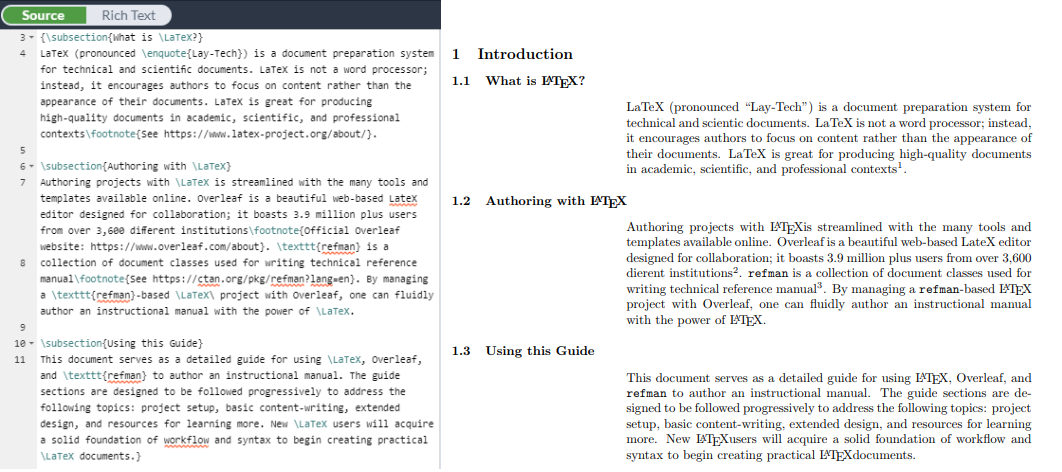
\includegraphics[width=\linewidth]{graphics/IntroSource.png}
\par
\texttt{refman} is a collection of document classes used for writing technical reference manual\footnote{See https://ctan.org/pkg/refman?lang=en}. By managing \texttt{refman}-based projects with Overleaf, authors can fluidly create instructional manuals with the power of \LaTeX.

\subsection{Using this Guide}
This document serves as a detailed guide for using \LaTeX, Overleaf, and \texttt{refman} to author an instructional manual. The guide sections are designed to be followed progressively to address the following topics: project setup, basic content-writing, extended design, and resources for learning more. New \LaTeX\ users will acquire a solid foundation of workflow and syntax to begin creating practical \LaTeX\ documents.}